\subsection{The Model}
	The following model concerns the most characterizing features of the system. We avoided to burden the model with trivial and non-significant details.
	
	\subsubsection*{Data Types}
		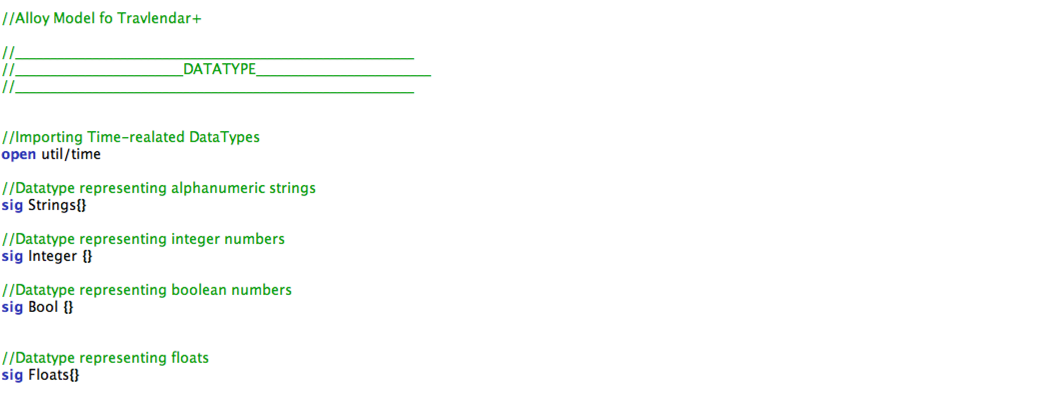
\includegraphics[width = \textwidth]{alloy/code/dataType}

	\subsubsection*{Signatures}
		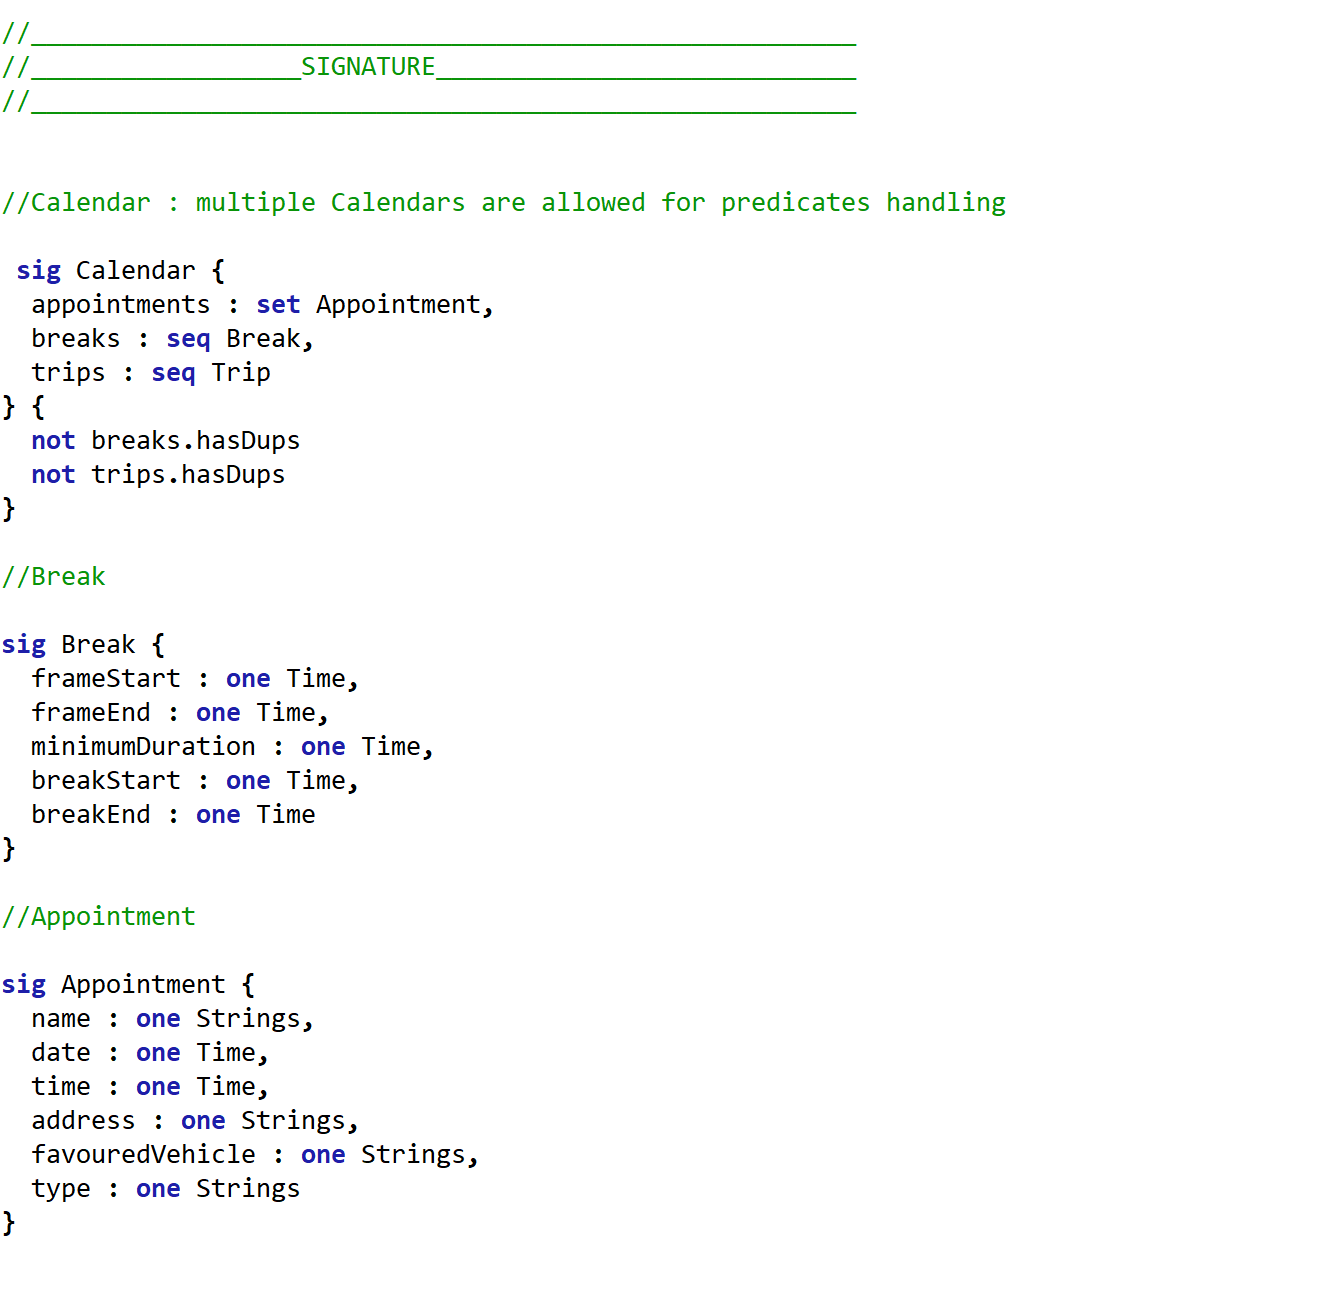
\includegraphics[width = \textwidth]{alloy/code/signature1}
		\vfill
		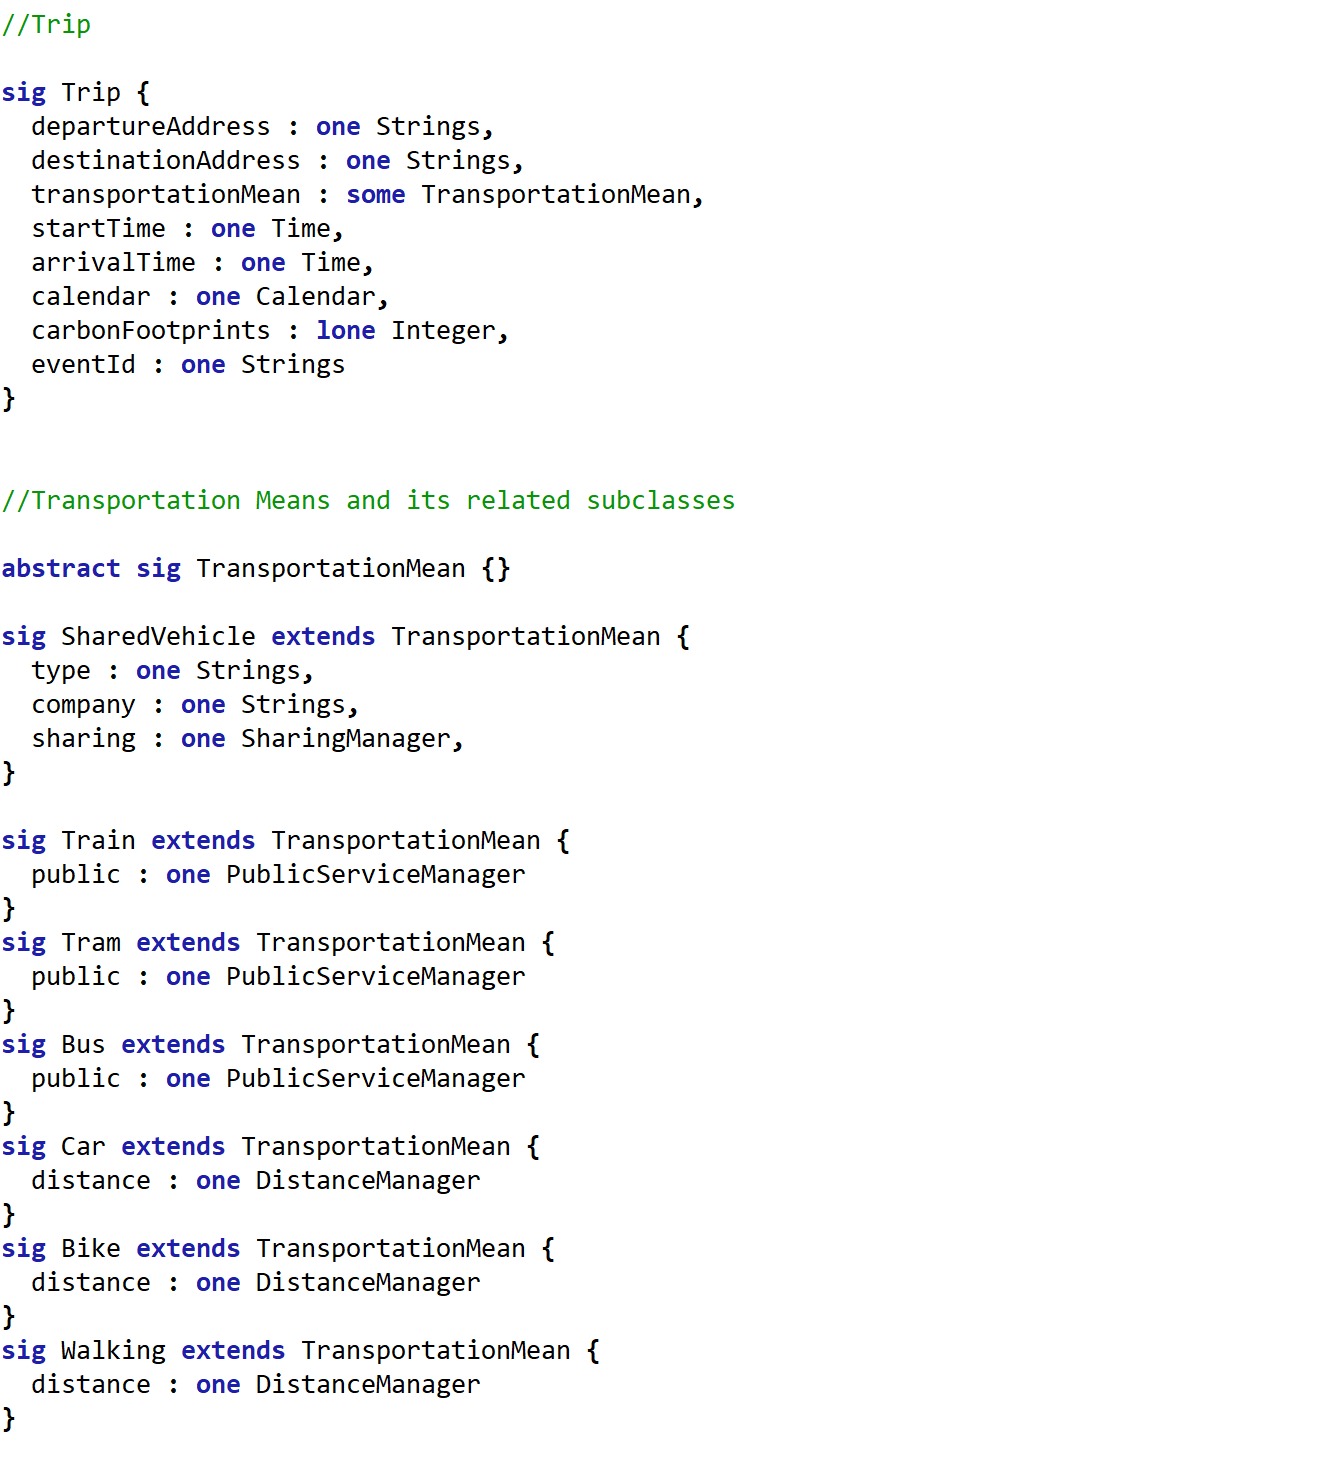
\includegraphics[width = \textwidth]{alloy/code/signature2}
		\vfill
		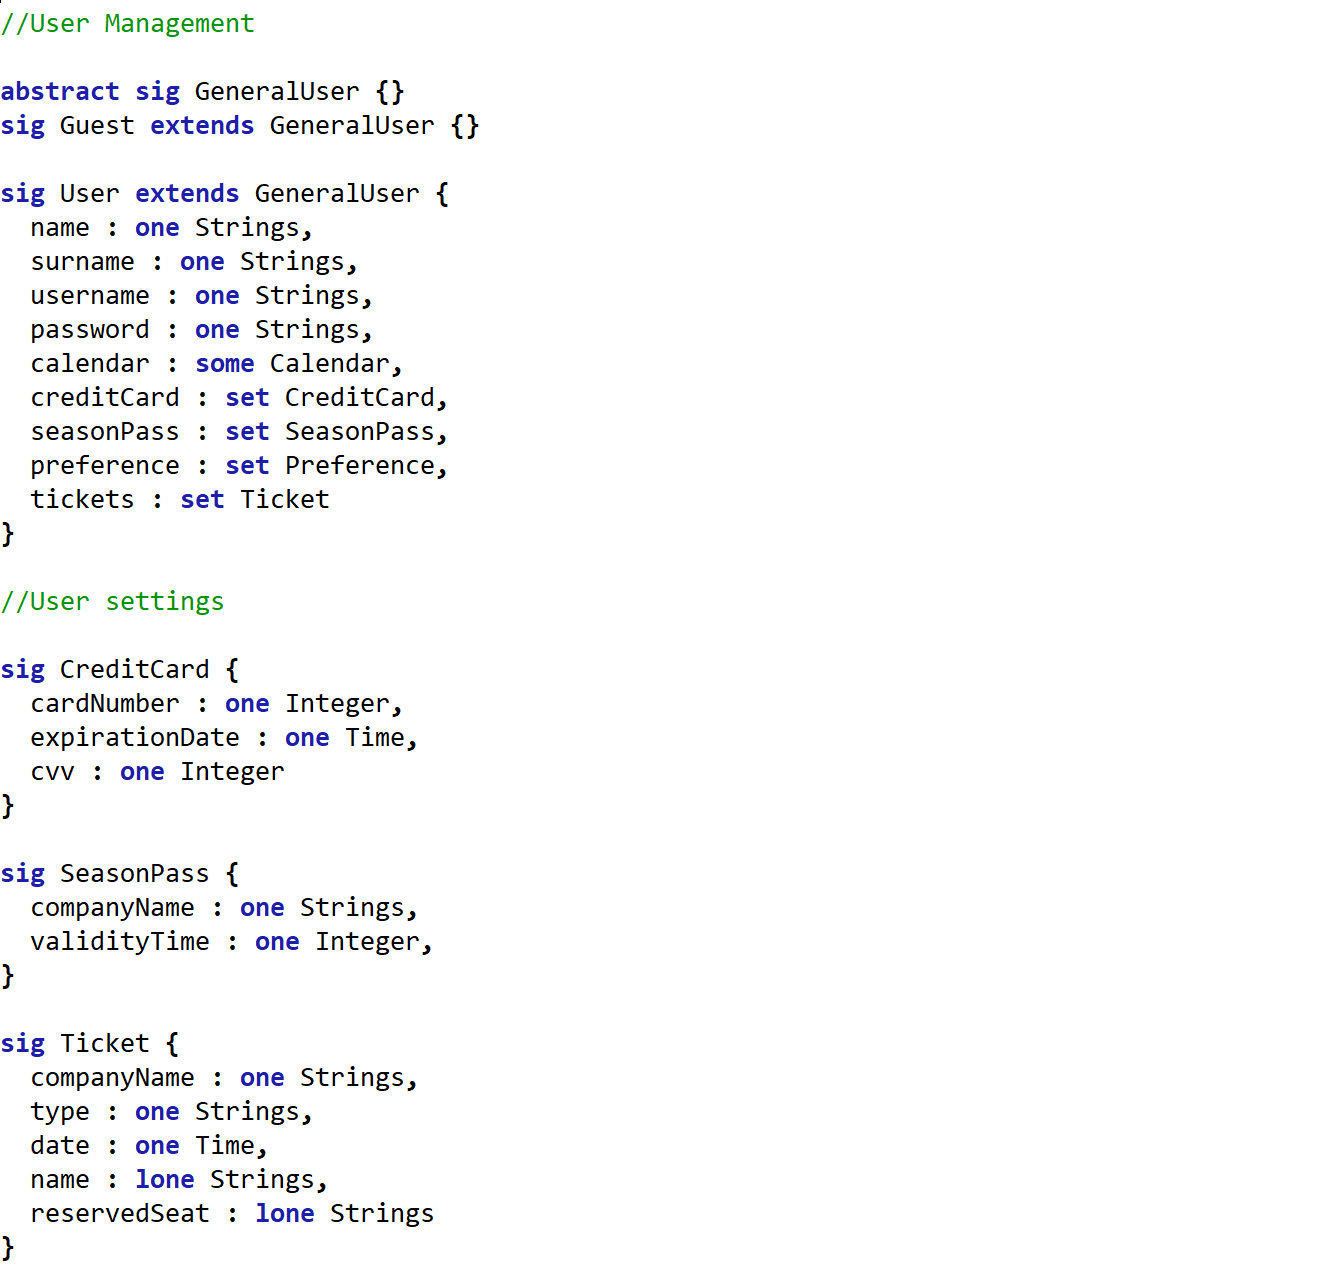
\includegraphics[width = \textwidth]{alloy/code/signature3}
		\bigskip
	
	\subsubsection*{Facts}
		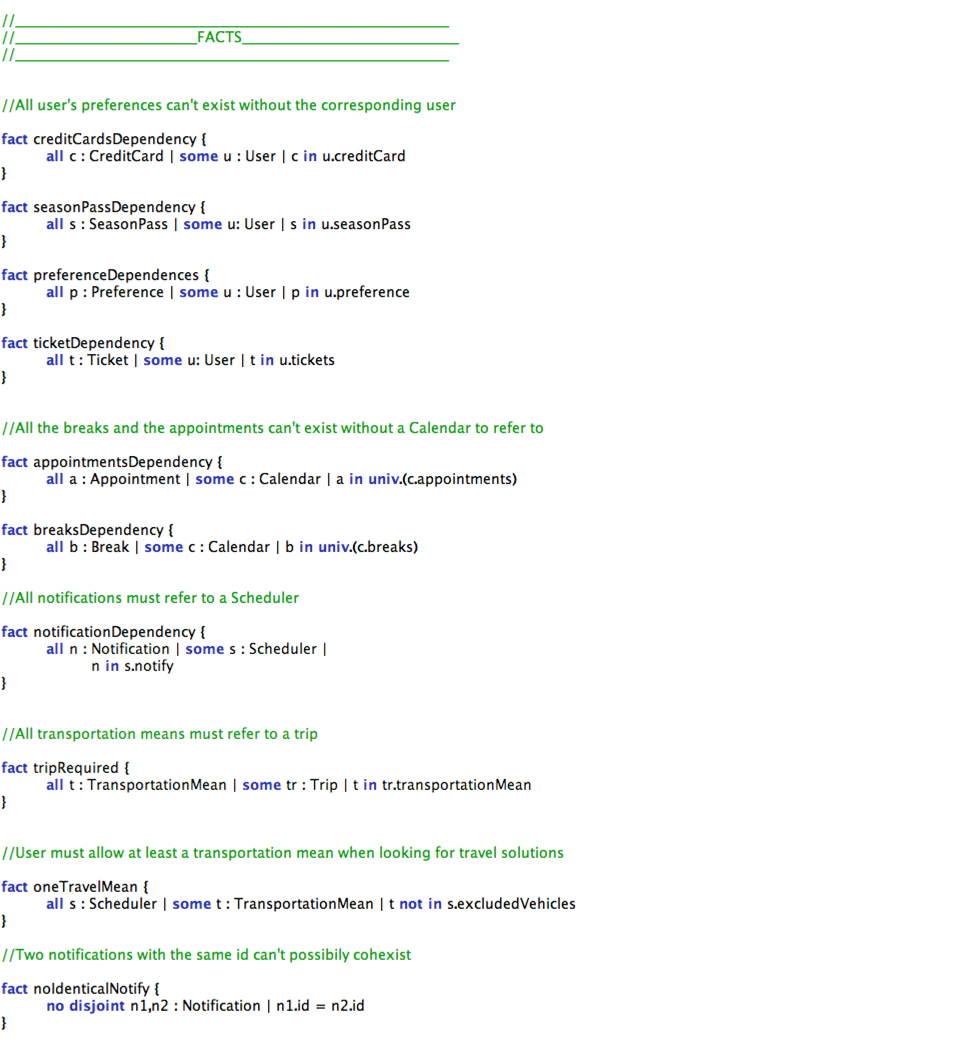
\includegraphics[width = \textwidth]{alloy/code/fact1}
		\vfill
		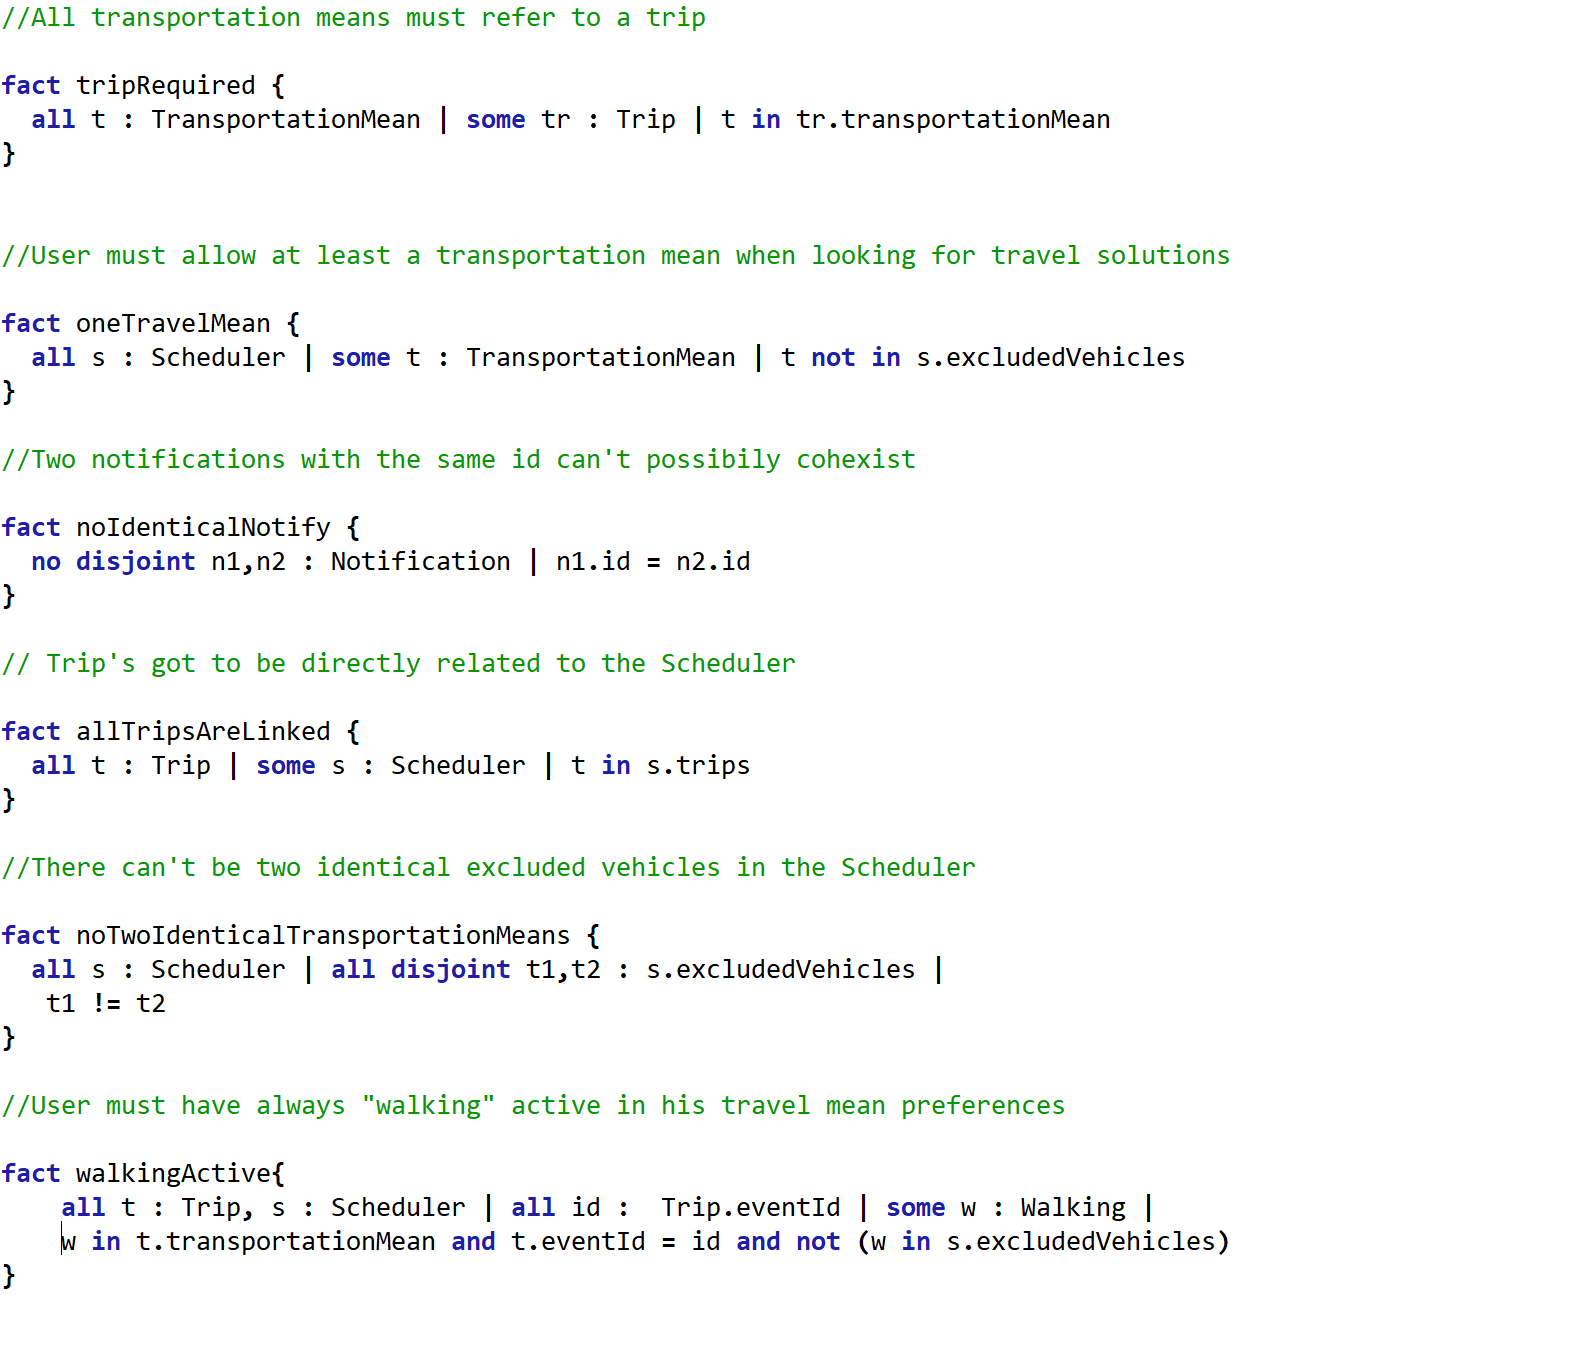
\includegraphics[width = \textwidth]{alloy/code/fact2}
		\bigskip
	
	\subsubsection*{Predicates}
		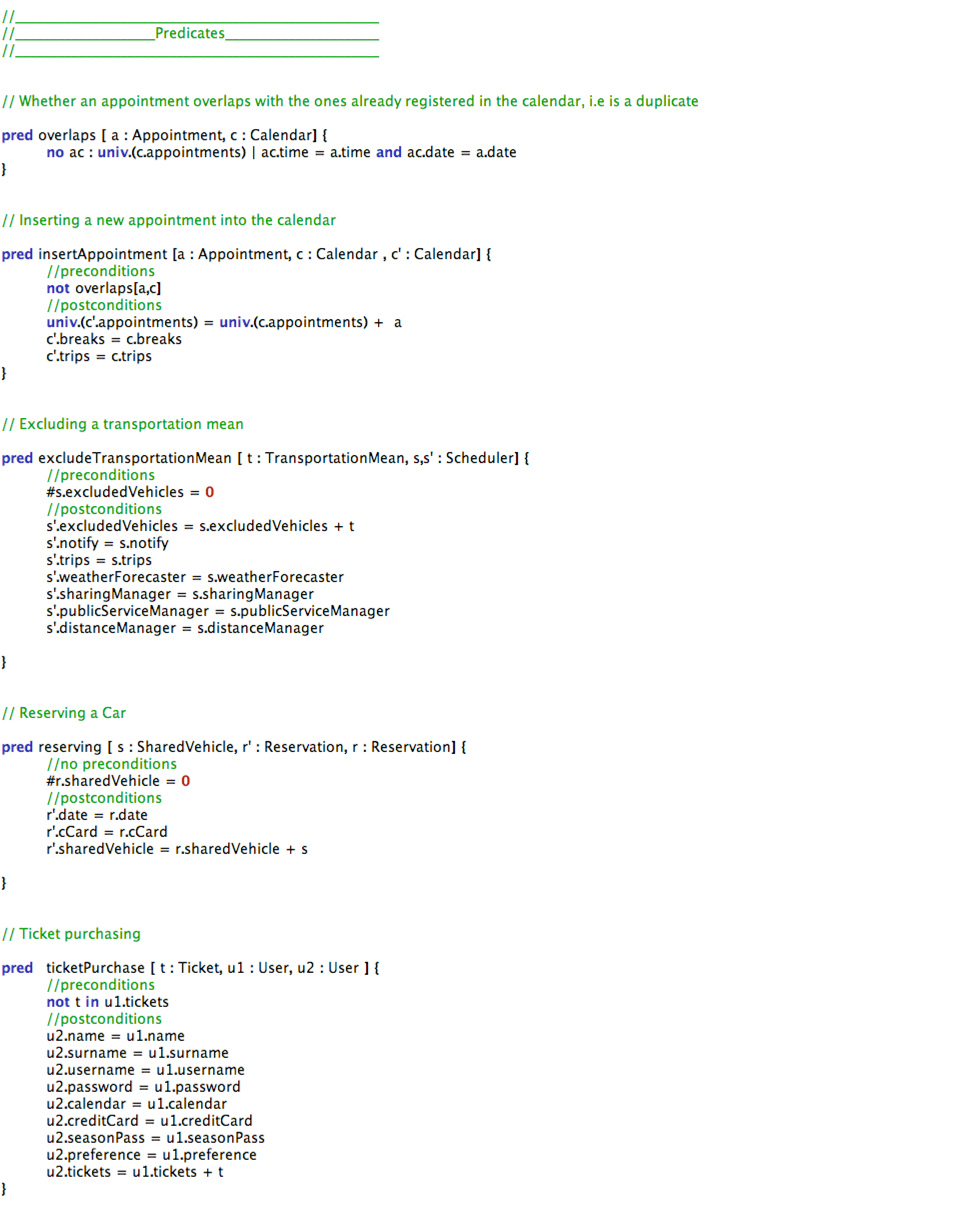
\includegraphics[width = \textwidth]{alloy/code/predicates}
		\bigskip
		
		
\subsection{Results}
	\begin{figure}[H]
		\centering
		
\includegraphics[width = 0.7\linewidth]{alloy/generatedWorld/alloyResult}
		\caption{Result of the model analysis.}		
		\label{fig:alloyResult}
	\end{figure}
	\bigskip
	
	
\subsection{Generated World}

	\begin{landscape}
		\subsubsection{World Generated}
			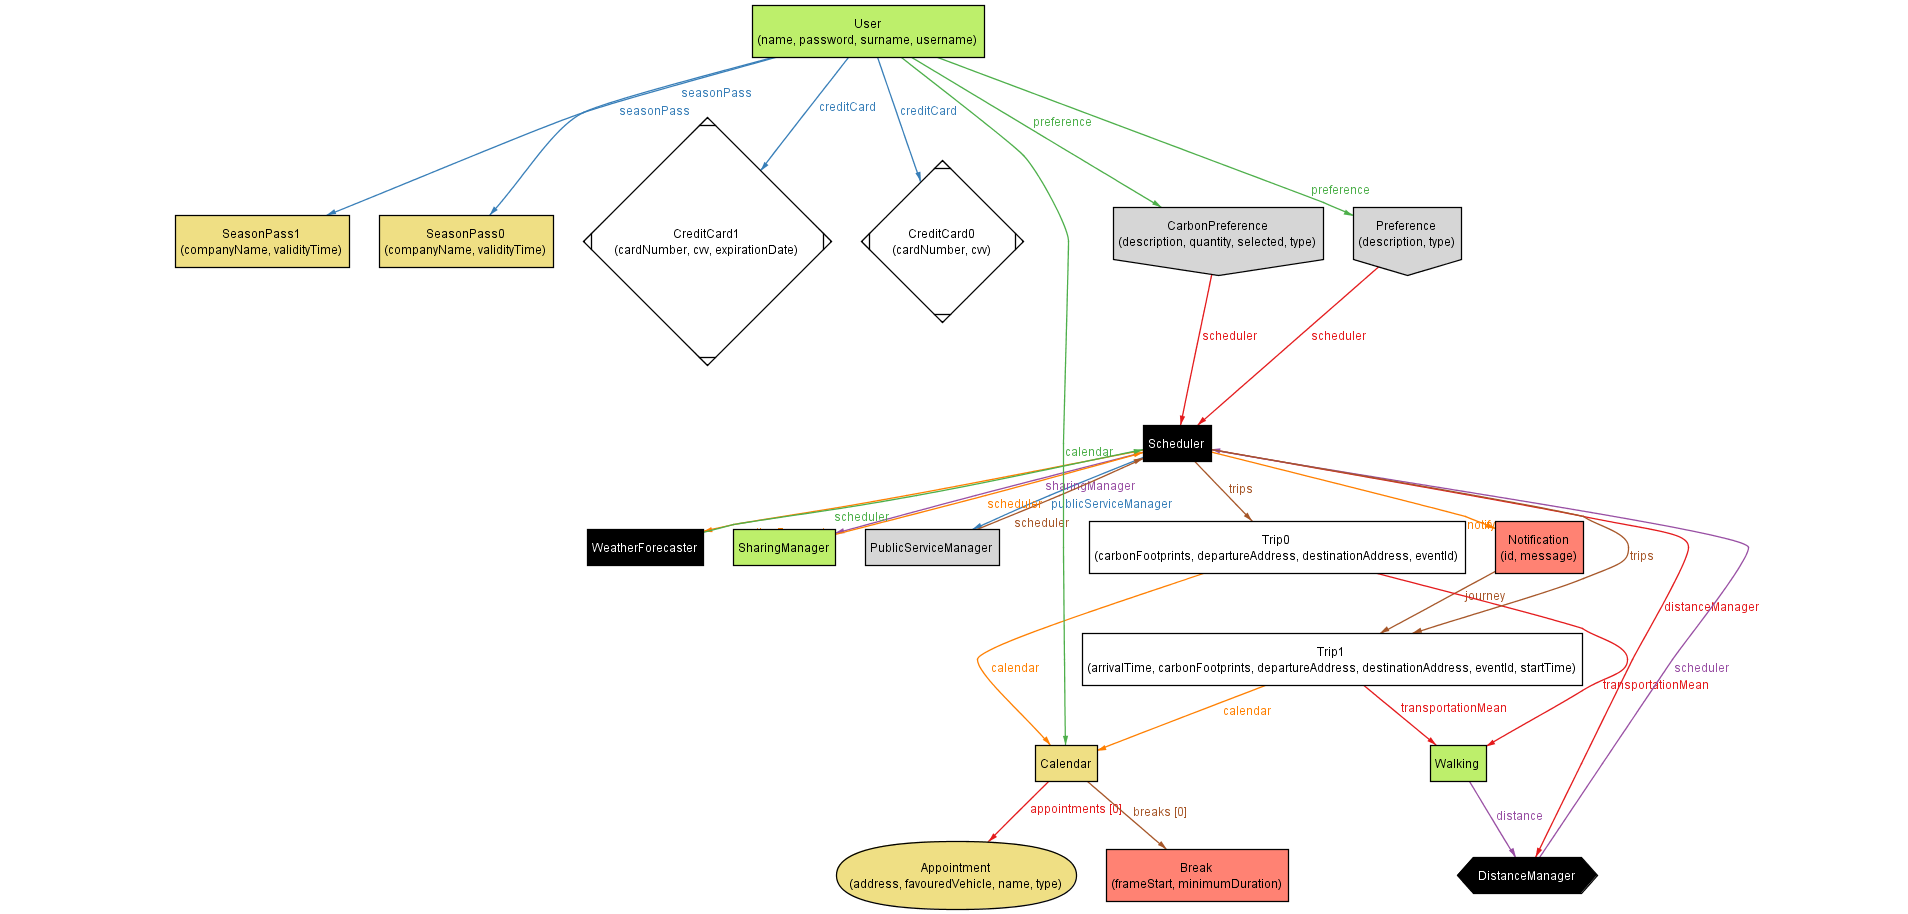
\includegraphics[height= \textheight , center]{alloy/generatedWorld/WorldGenerated}
	
		\subsubsection{Ticket Purchase}
			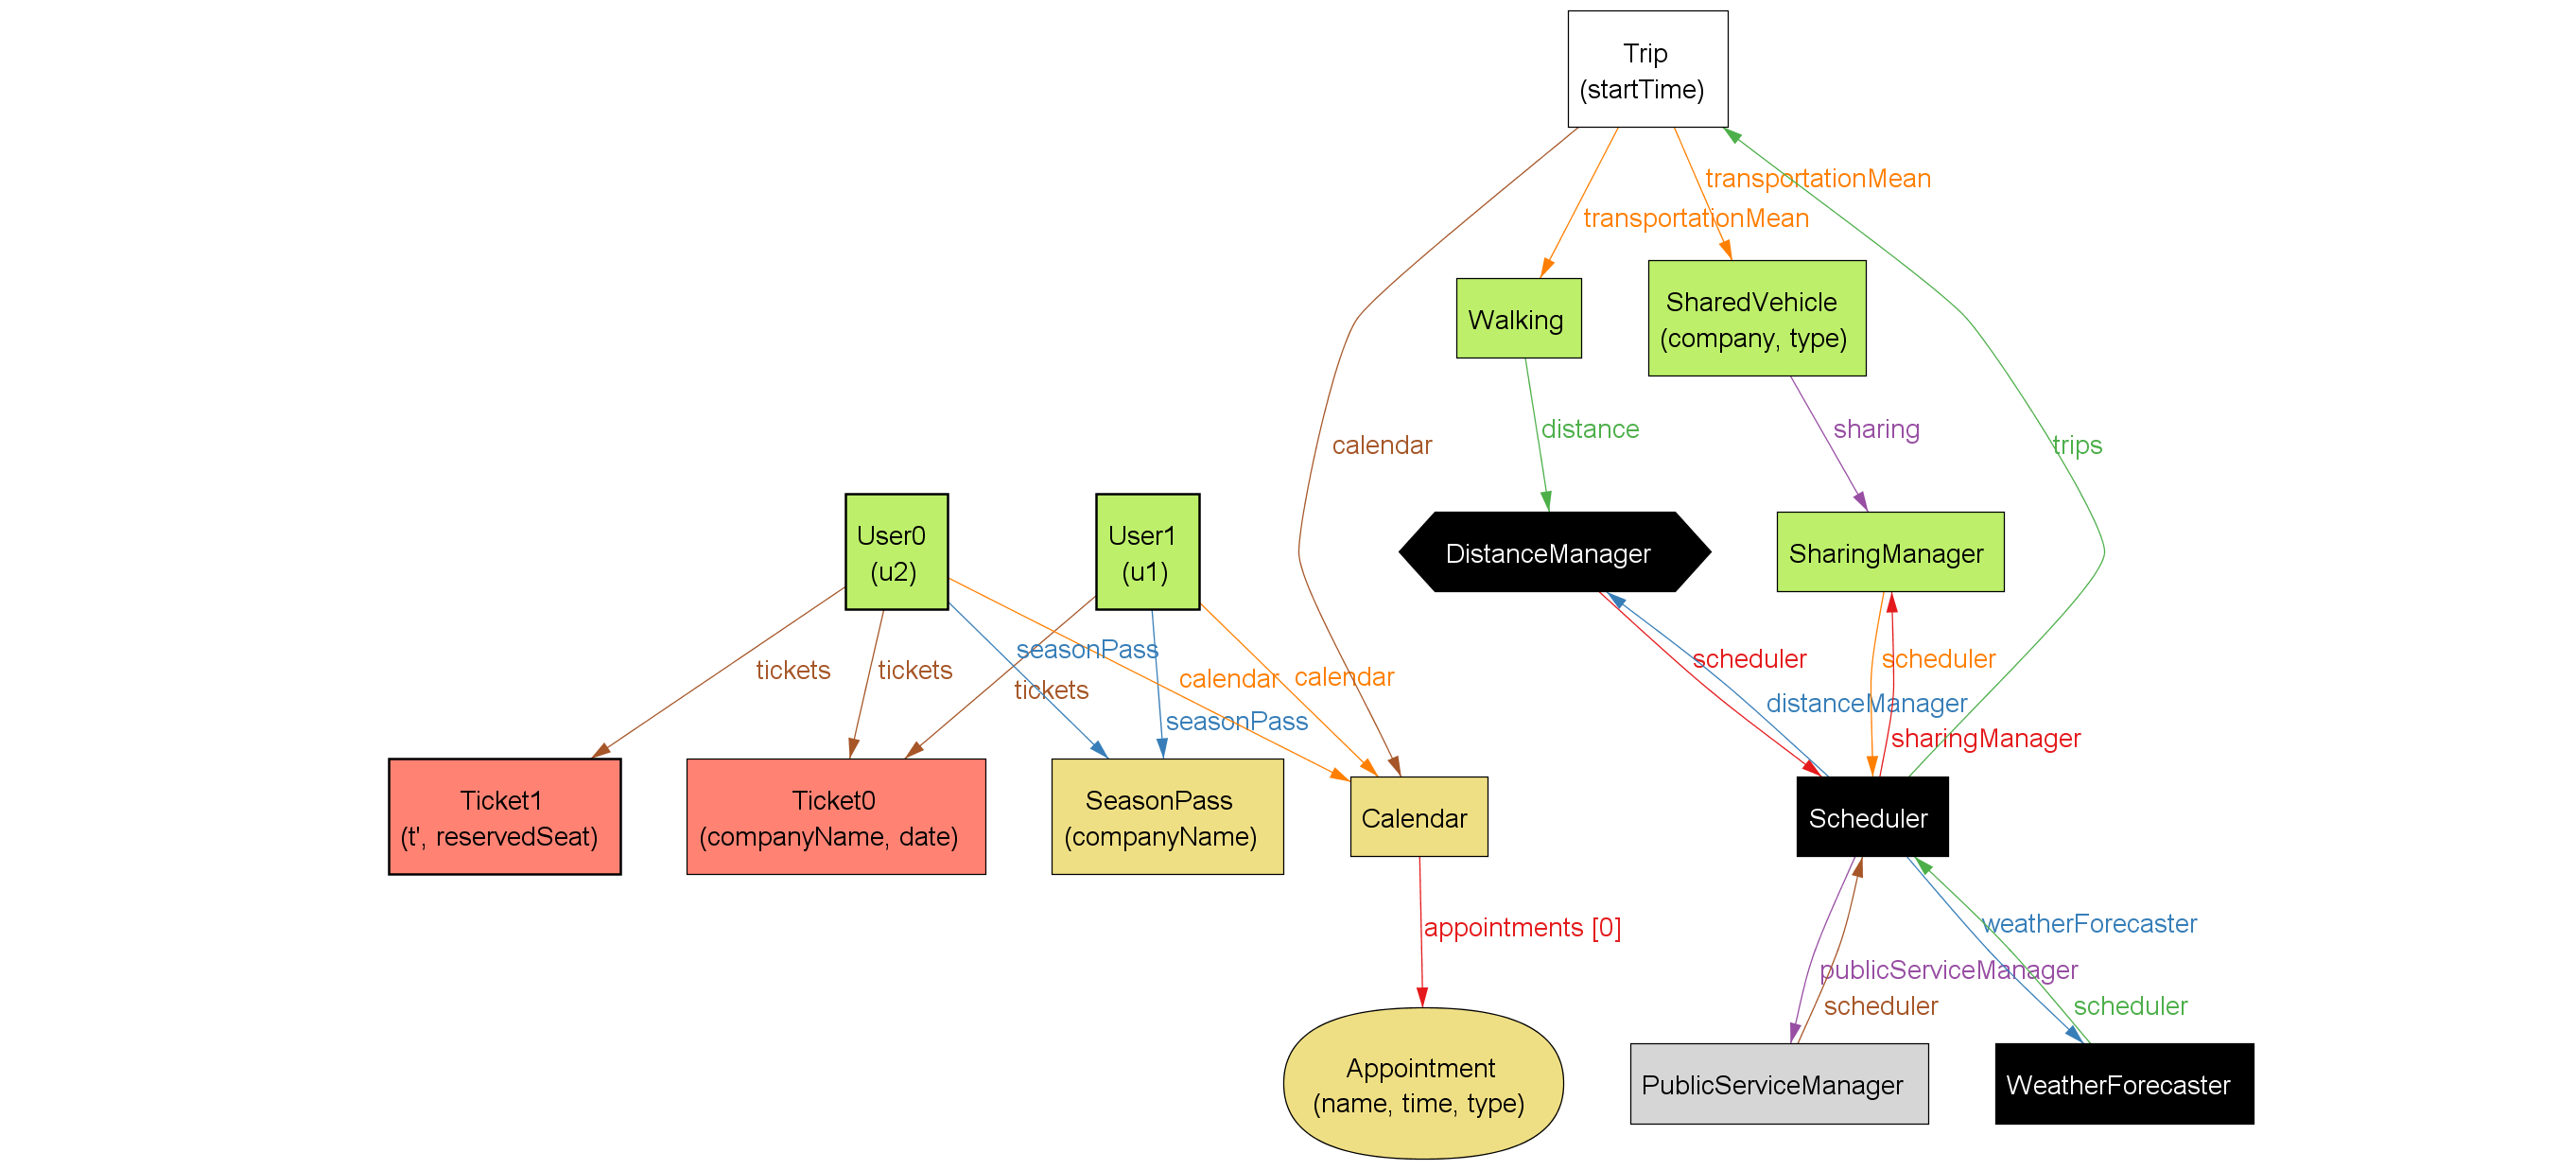
\includegraphics[height= \textheight, center]{alloy/generatedWorld/ticketPurchase}
	
		\subsubsection{Renting}
			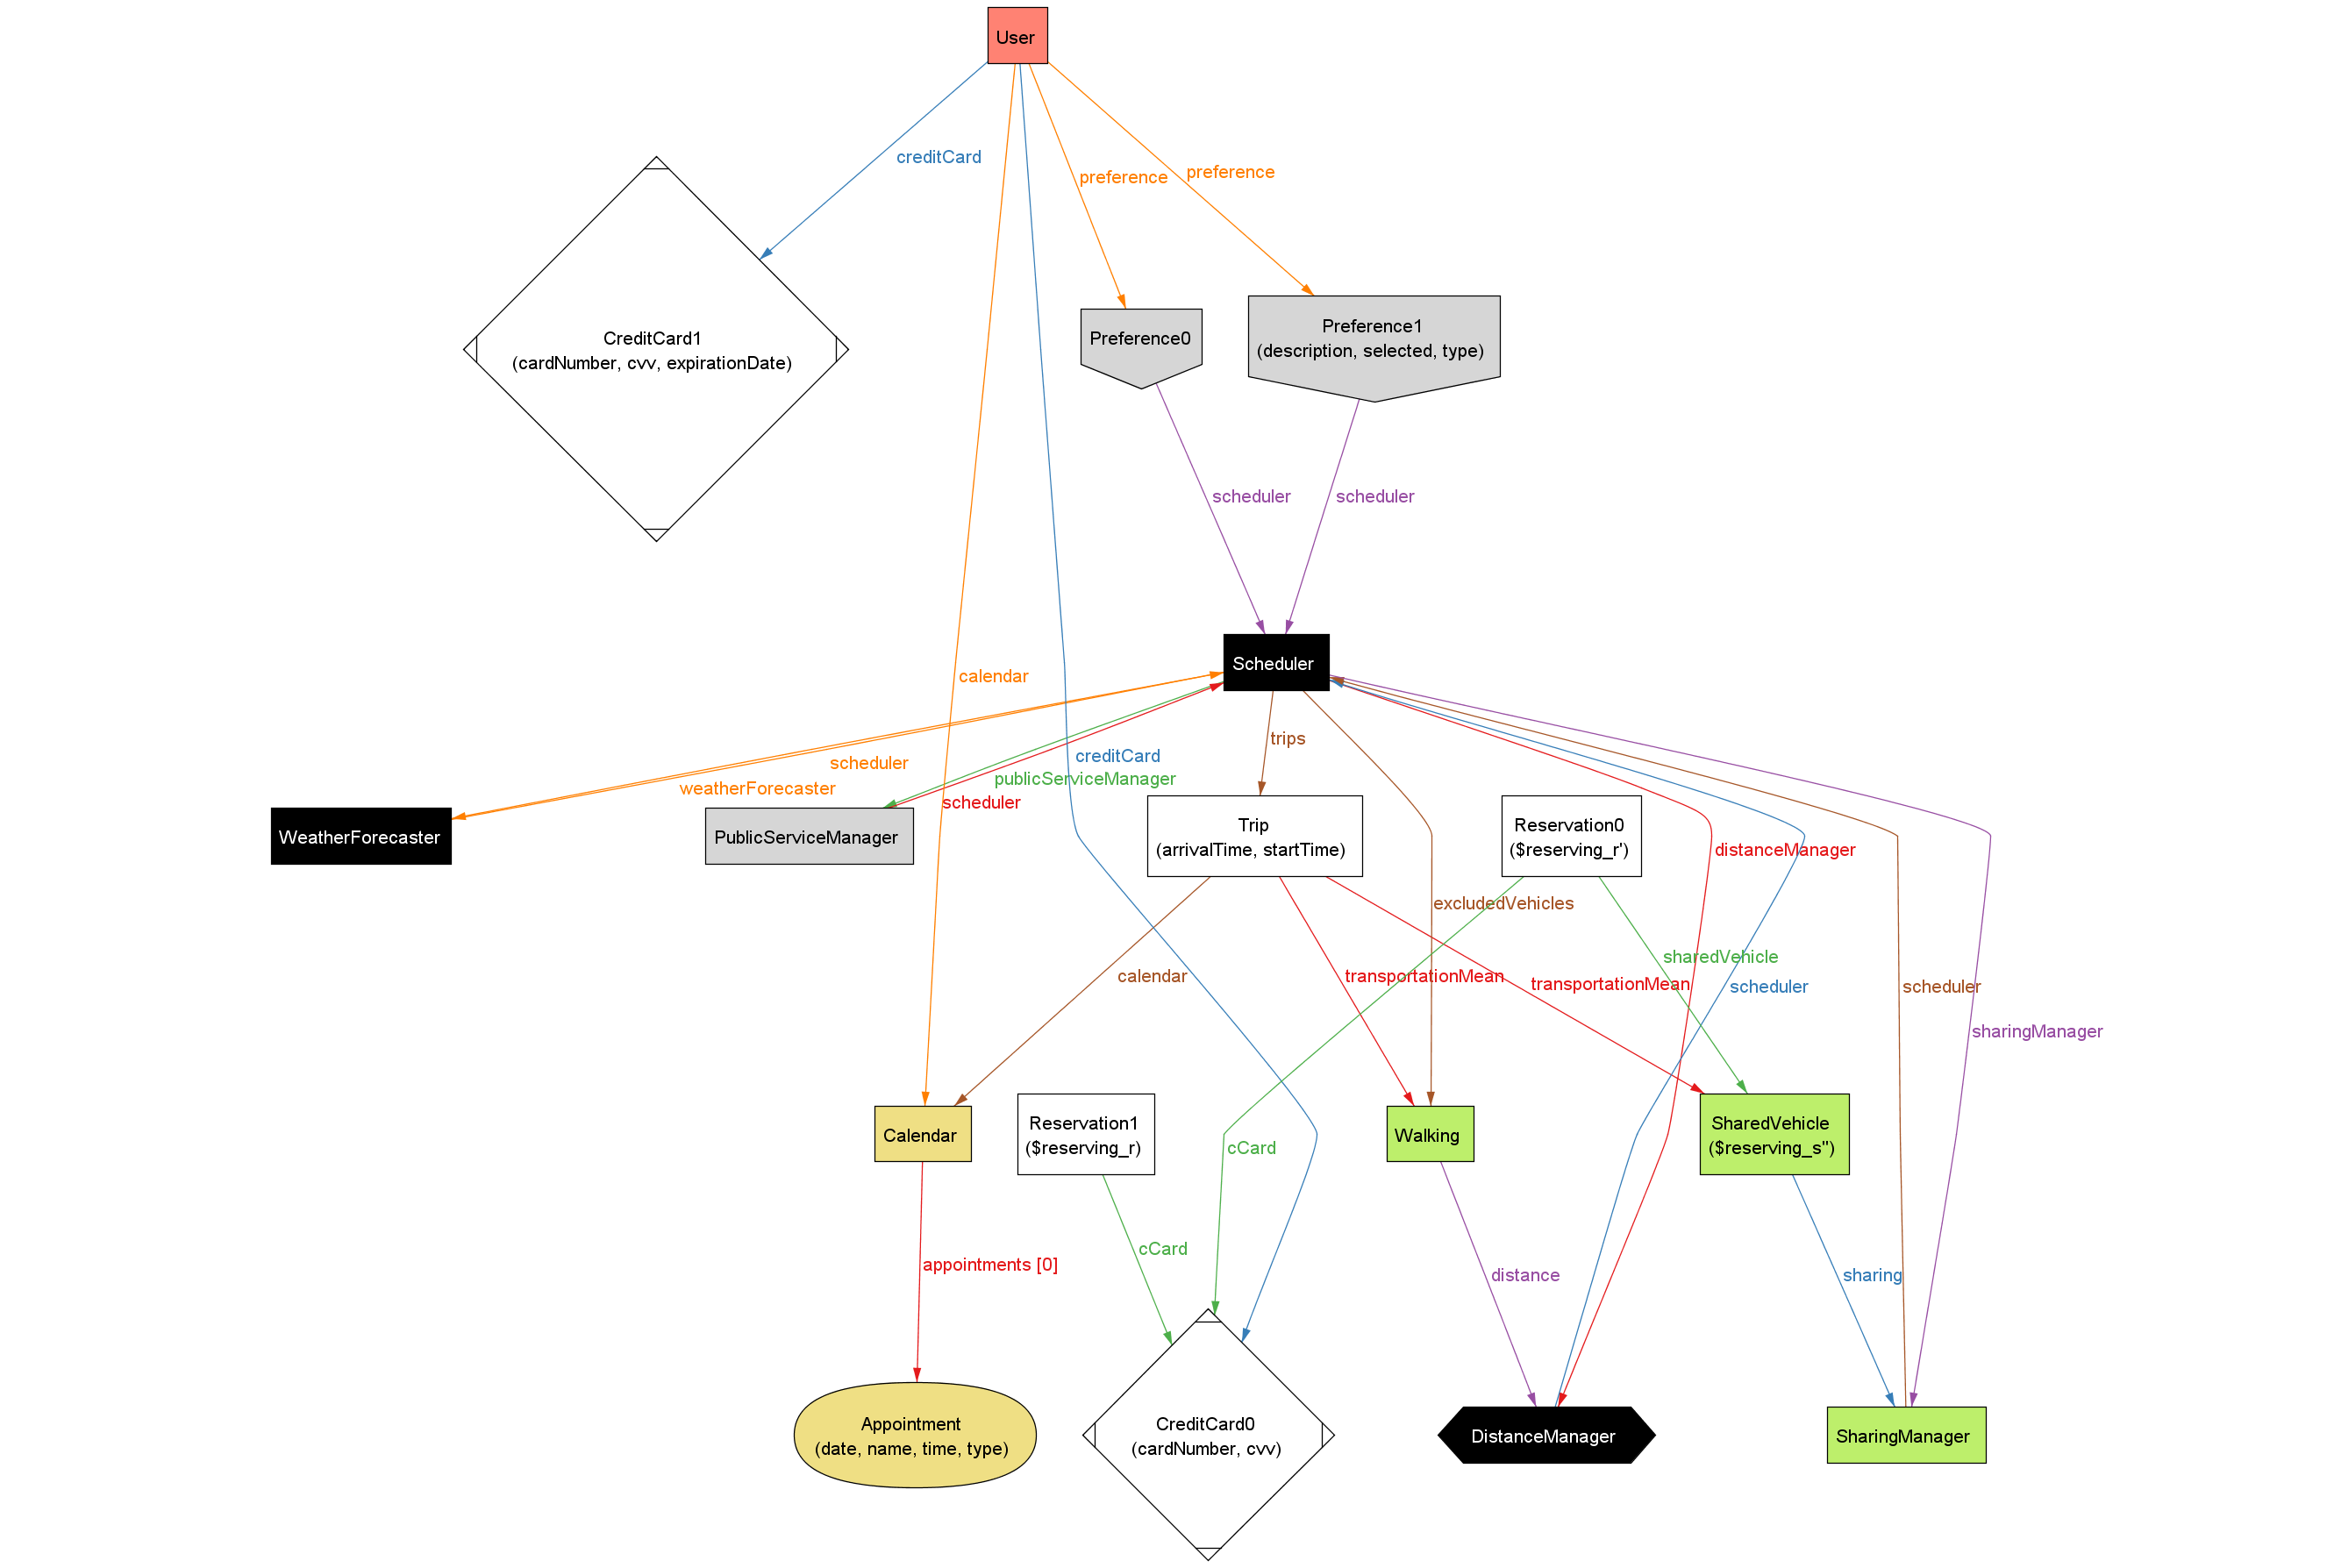
\includegraphics[height = \textheight, center]{alloy/generatedWorld/renting}
		
		\subsubsection{Insert Appointment}
			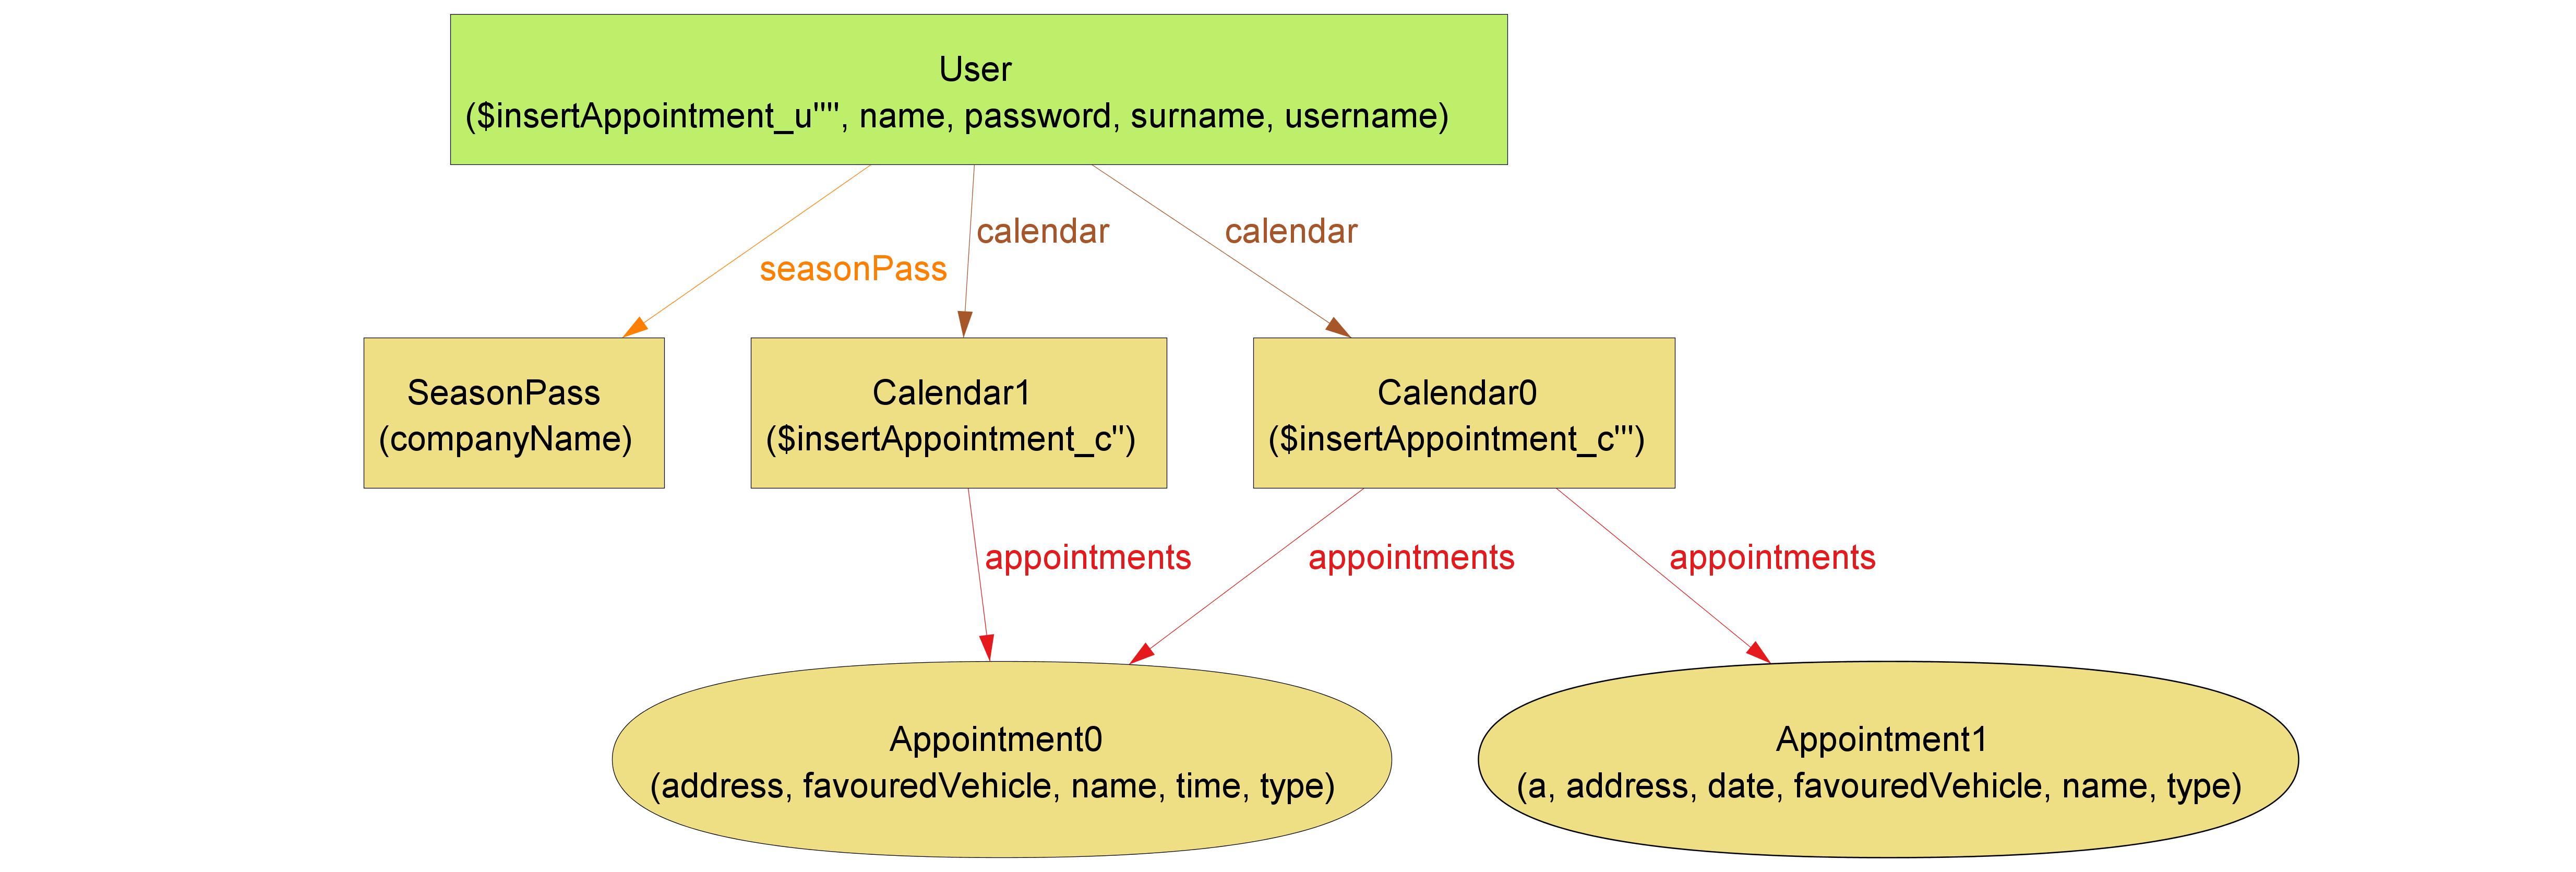
\includegraphics[height = \textheight, center]{alloy/generatedWorld/insertAppointment}
	\end{landscape}
	